\documentclass{article}
\usepackage{multirow}
\usepackage{geometry}
\usepackage{fancyhdr}
\usepackage{outlines}
\usepackage{tocloft}
\usepackage{graphicx}
\graphicspath{ {./images/} }
\usepackage{subcaption}
\usepackage[hidelinks]{hyperref}
\hypersetup{
    colorlinks,
    citecolor=black,
    filecolor=black,
    linkcolor=black,
    urlcolor=black
}
\geometry{
	margin=1in
}

\pagestyle{fancy}
\fancyhf{}
\lhead{Maximizing OU Student Success by Predicting Student Failure\\CS773 Capstone Project}
\rfoot{Page \thepage}
\rhead{Alex Launi\\Old Dominion University}

\title{Maximizing OU Student Success by Predicting Student Failure\\ \rule{\textwidth}{0.5pt}\\CS773 Capstone project}
\author{Alex Launi\\Old Dominion University\\01124306}
\date{Summer 2019}

\renewcommand\cftsecfont{\normalfont}
\renewcommand\cftsecpagefont{\normalfont}
\renewcommand{\cftsecleader}{\cftdotfill{\cftsecdotsep}}
\renewcommand\cftsecdotsep{\cftdot}
\renewcommand\cftsubsecdotsep{\cftdot}

\begin{document}
\maketitle
\tableofcontents
\listoffigures

\pagebreak
\section{Executive Summary}
The objective of this project is to develop models that can predict student success
within a course module so that educators can intervene at the earliest indications of
trouble, to help prevent said student from failing, or withdrawing from the course.\\
Two types of data are used to achieve this goal.
\begin{itemize}
	\item Student demographic data
	\item Student-VLE interaction data
\end{itemize}

\section{Introduction}
Education is of prime importance for economic mobility. Broadband internet has made
it possible for quality educational products to be made available to a much wider swath
of the population. Traditionally, at least in the United States, educational resources were not
distributed equally to all individuals. Numerous studies have shown the correlation
between zip code, economic mobility, and quality of education. The possibility of delivering
high quality education products to students in disparate areas is very exciting. In order to
maximize the potential gain this system has to offer I have developed predictive models
that will enable administrators, educators, and mentors the ability to identify students who
are at an elevated risk of not completing their module so that an intervention may be conducted
and the student guided back to success.\\

The Open University (OU) is open to students regardless of previous educational history, and offers
hundreds of distance learning courses. The virtual learning environment is the portal through which OU
students interact with the course materials, much in the way that Blackboard and PLE function for ODU
online students. Students are grouped into small class sizes and a teaching assistant is assigned to provide
help, grade assignments, and guide the cohort through the course.\\

A reliable means to identify at-risk students before too much
damage is done would be a major boon the success of the program as a whole. An online program could potentially 
have many more students than traditional classroom based programs. The cost of too many interventions could be 
prohibitively high, and many may be false positives; worse there may be many false negatives.

\section{Problem Statement}
Our goal is to identify students who need some form of intervention so that teaching assistants, and OU
 administration can best target intervention to the students for whom it will have the most impact. To achieve
 this goal we attempt to utilize student demographics, course interaction data, and student performance data for
 students in the same course.

\section{Methodology}
This project used the anonymized Open University Learning Analytics Dataset (OULAD). The data was collected by the Open University to help optimize learning materials. It is comprised of student demographics, assessment results, and click-stream data for over 32,000 students across 22 courses. 1,111 entries had missing values of imd\_band. Instances with missing data were removed from the dataset. 3,516 entries with imd\_band ``10-20`` were relabelled ``10-20\%`` for consistency. The criterion for \texttt{at risk} was considered in 2 distinct groups and the experiments were run independently to see if failure and drop out could be treated as one, or if they were distinct variants of students in need of help. For each model Stratified 5-fold cross validation was performed. Models were evaluated based on F-measure, precision, recall, and accuracy. Scores reported are the mean of the 5 runs.\\

\subsection{Learning Models}
In this project 4 machine learning models were employed. Decision Tree classification, Logistic Regression classification, Random Forest, and Support Vector Machines. All models were implemented in Python using models from the scikit-learn library both for preprocessing, and learning. Feature engineering was performed both by intuition gained from exploratory data analysis, and with scikit-learn's recursive feature elimination. No significant difference in predictive ability of the models was observed between these two methods, validating the conclusions reached during data analysis.

\subsubsection{Decision Tree Classification}
Decision tree classification was performed with the \texttt{sklearn.trees.DecisionTree} class. No hyperparameter optimization was performed with the exception of \texttt{max\_depth} hyperparameter which was set to \texttt{max\_depth = 3} in order to reduce the tree to a size conducive to printing for visualization purposes. Splits were performed based on feature entropy.

\subsubsection{Random Forest}
Random forest was performed in an indentical fashion to the decision tree model with the exception that sklearn's RFE class was used in lieu of features selected during EDA.

\subsubsection{Logistic Regression}
Logistic regression was performed both on demographic data, and VLE interaction data. Feature scaling was attempted, but no change in prediction power was observed.

\subsubsection{SVM}
SVM using the radial basis function kernel was performed on VLE interaction data and results compared to logistic regression.

\subsection{Failure and Withdrawn \texttt{at risk}}
\begin{figure}[ht!]
	\centering
	\begin{subfigure}{.45\textwidth}
		\centering
		\fbox{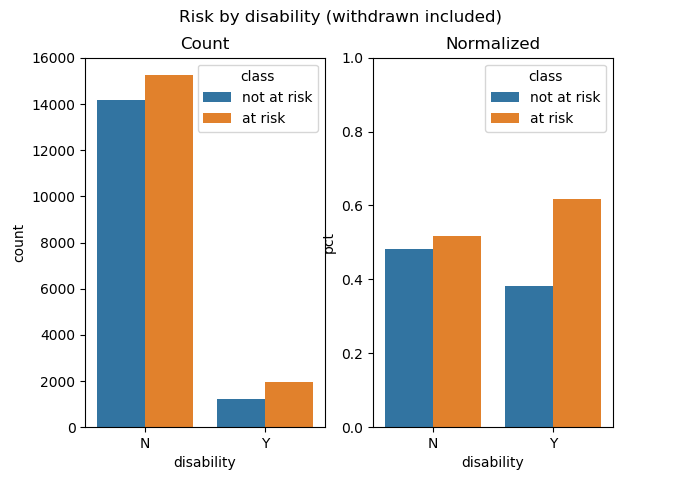
\includegraphics[width=0.8\textwidth]{EDA/withdrawn_at_risk/risk_by_disability_combined.png}}
		\caption{Risk by disability, count and normalized}
		\label{fig:risk_by_dis_all}
	\end{subfigure}
	\begin{subfigure}{.45\textwidth}
		\centering
		\fbox{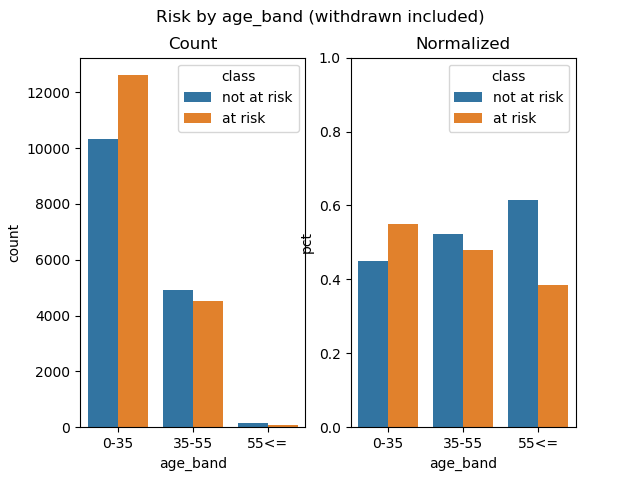
\includegraphics[width=0.8\textwidth]{EDA/withdrawn_at_risk/risk_by_age_band_combined.png}}
		\caption{Risk by age band, count and normalized}
		\label{fig:risk_by_age_all}
	\end{subfigure}
		\begin{subfigure}{.45\textwidth}
		\centering
		\fbox{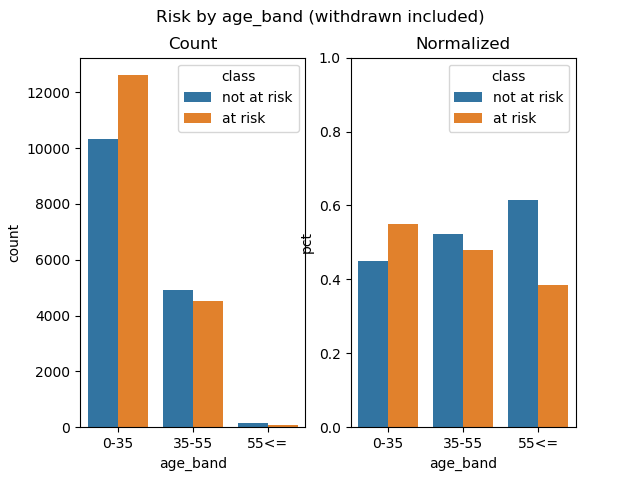
\includegraphics[width=0.8\textwidth]{EDA/withdrawn_at_risk/risk_by_age_band_combined.png}}
		\caption{Risk by age band, count and normalized}
		\label{fig:risk_by_age_all}
	\end{subfigure}
	\begin{subfigure}{.45\textwidth}
		\centering
		\fbox{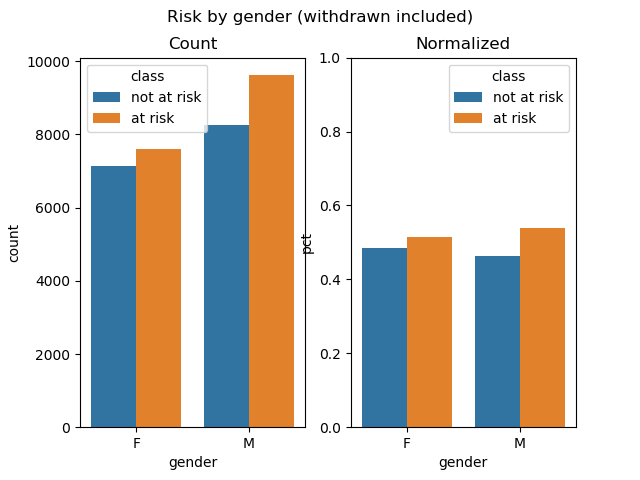
\includegraphics[width=0.8\textwidth]{EDA/withdrawn_at_risk/risk_by_gender_combined.png}}
		\caption{Risk by gender, count and normalized}
		\label{fig:risk_by_gender_all}
	\end{subfigure}

	\begin{subfigure}{.45\textwidth}
		\centering
		\fbox{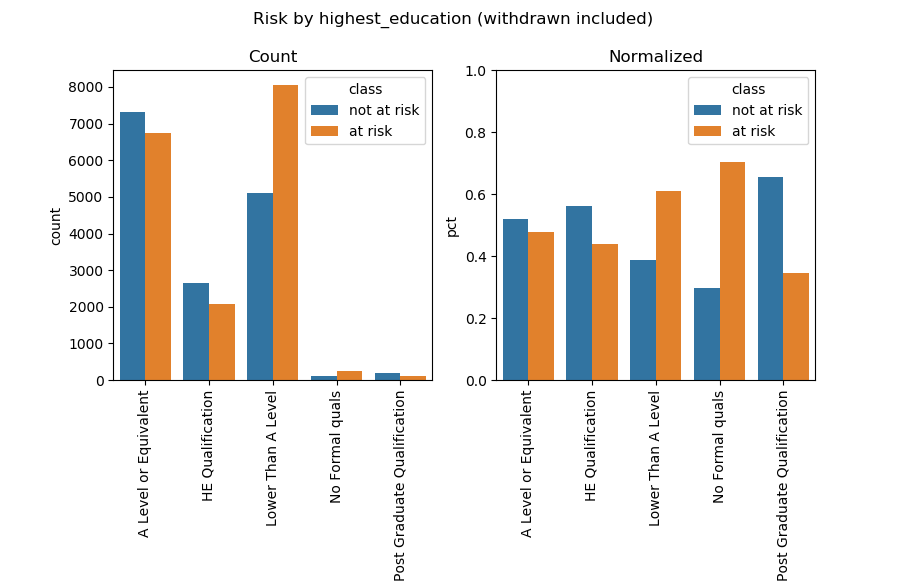
\includegraphics[width=0.8\textwidth]{EDA/withdrawn_at_risk/risk_by_highest_ed_combined.png}}
		\caption{Risk by highest education level, count and normalized}
		\label{fig:risk_by_ed_all}
	\end{subfigure}
	\begin{subfigure}{.45\textwidth}
		\centering
		\fbox{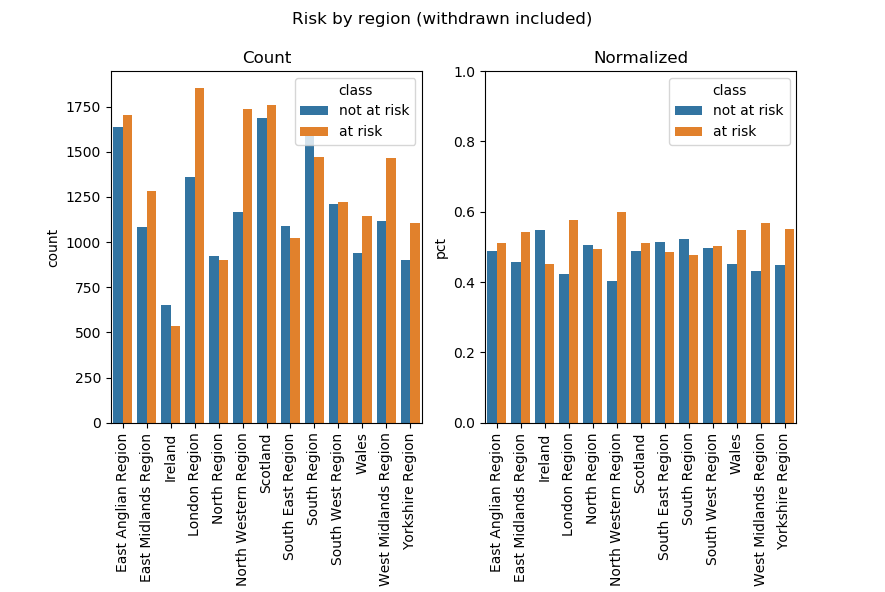
\includegraphics[width=0.8\textwidth]{EDA/withdrawn_at_risk/risk_by_region_combined.png}}
		\caption{Risk by region, count and normalized}
		\label{fig:risk_by_region_all}
	\end{subfigure}
	\caption{Risk by feature for all \texttt{at risk} students}
	\label{fig:feature_risk_all}
\end{figure}

The data were evaluated for any obvious connection between feature and risk, both as raw counts and as normalized values. This analysis yielded disability, education level, and region as potentially strong demographic indicators of risk. Relationship between feature and risk for data with withdrawn students is shown as raw count, and in normalized form in Figure \ref{fig:feature_risk_all}.

\begin{figure}[ht!]
	\centering
	\fbox{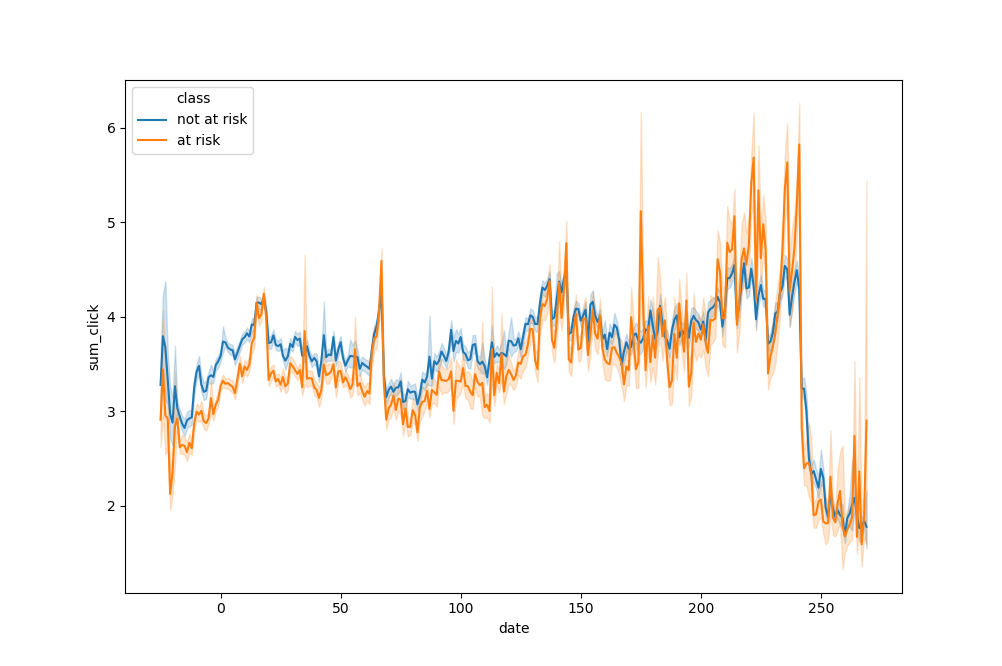
\includegraphics[width=0.8\textwidth]{EDA/withdrawn_at_risk/clicks_per_day.png}}
	\caption{Mean clicks per day (withdrawn at risk)}
	\label{fig:clicks_per_day_all}
\end{figure}
Student activity was evaluated as a predictor of success. The activity level of students who passed courses showed a much narrower range per day. Students who failed or withdrew displayed lower amounts of activity, until the last portion of their courses where they exhibited a dramatic spike in activity, likely as an attempt to make up lost time (shown in Figure \ref{fig:clicks_per_day_all}).

\clearpage
\subsection{Only failure \texttt{at risk}}
\begin{figure}[h]
	\centering
	\begin{subfigure}{.45\textwidth}
		\centering
		\fbox{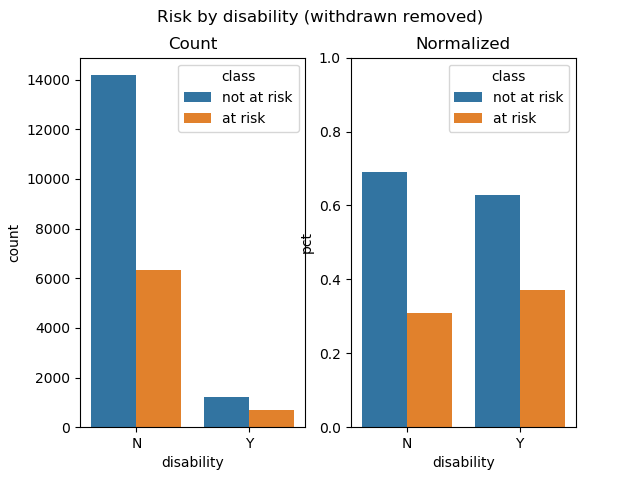
\includegraphics[width=0.8\textwidth]{EDA/withdrawn_not_at_risk/risk_by_disability_combined.png}}
		\caption{Risk by disability, count and normalized}
		\label{fig:risk_by_dis_nowd}
	\end{subfigure}
	\begin{subfigure}{.45\textwidth}
		\centering
		\fbox{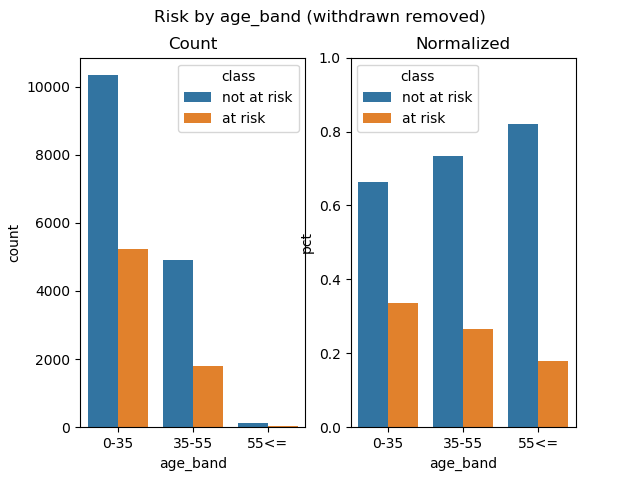
\includegraphics[width=0.8\textwidth]{EDA/withdrawn_not_at_risk/risk_by_age_band_combined.png}}
		\caption{Risk by age band, count and normalized}
		\label{fig:risk_by_age_nowd}
	\end{subfigure}
		\begin{subfigure}{.45\textwidth}
		\centering
		\fbox{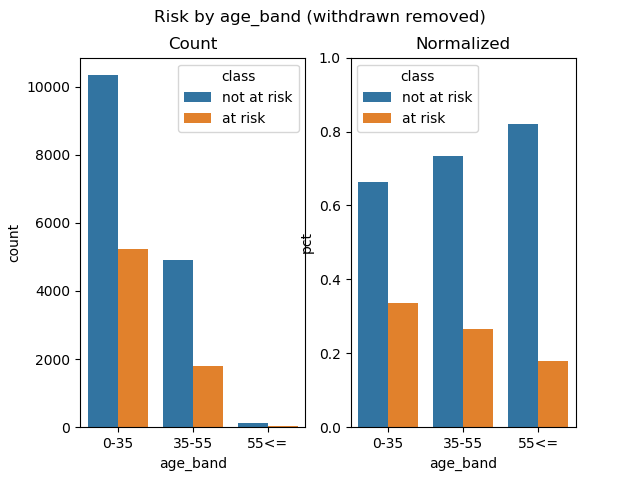
\includegraphics[width=0.8\textwidth]{EDA/withdrawn_not_at_risk/risk_by_age_band_combined.png}}
		\caption{Risk by age band, count and normalized}
		\label{fig:risk_by_age_nowd}
	\end{subfigure}
	\begin{subfigure}{.45\textwidth}
		\centering
		\fbox{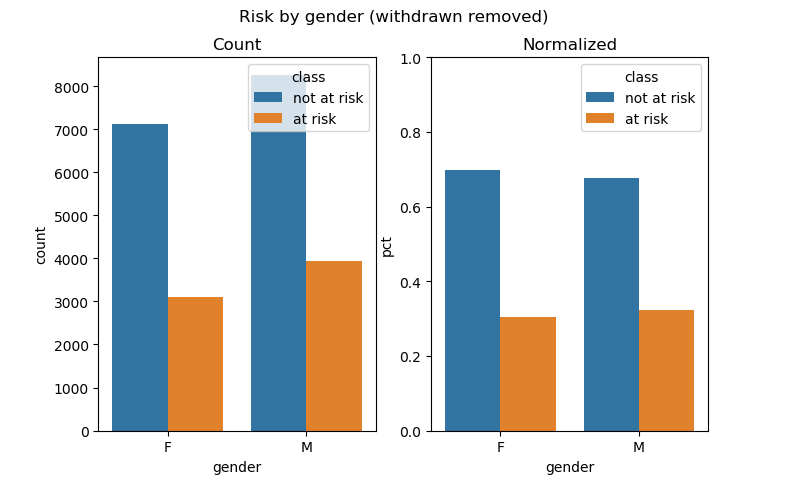
\includegraphics[width=0.8\textwidth]{EDA/withdrawn_not_at_risk/risk_by_gender_combined.png}}
		\caption{Risk by gender, count and normalized}
		\label{fig:risk_by_gender_nowd}
	\end{subfigure}

	\begin{subfigure}{.45\textwidth}
		\centering
		\fbox{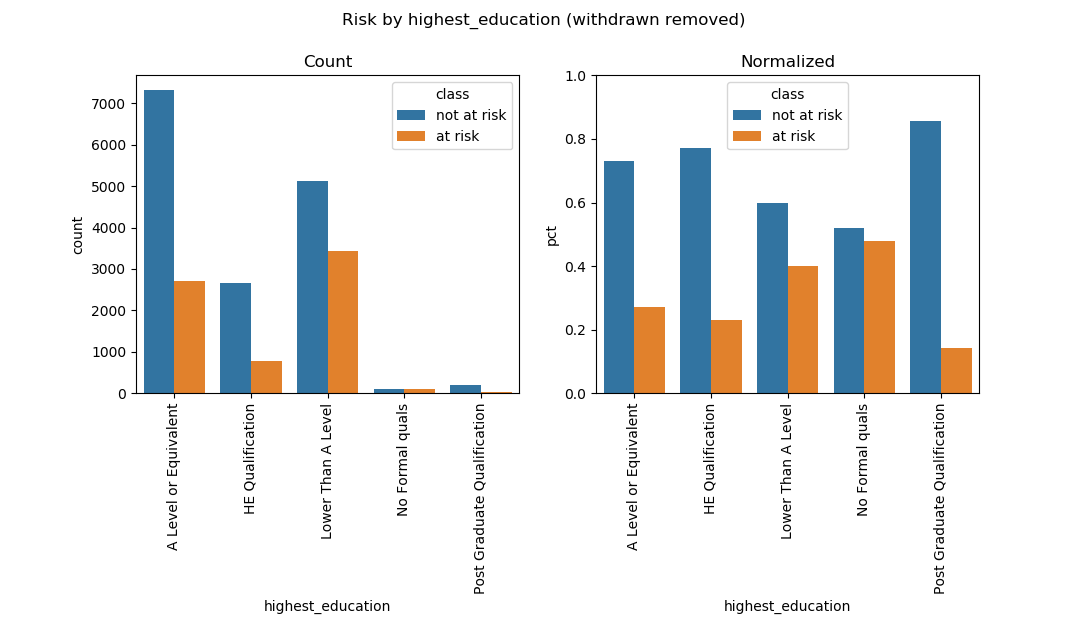
\includegraphics[width=0.8\textwidth]{EDA/withdrawn_not_at_risk/risk_by_highest_ed_combined.png}}
		\caption{Risk by highest education level, count and normalized}
		\label{fig:risk_by_ed_nowd}
	\end{subfigure}
	\begin{subfigure}{.45\textwidth}
		\centering
		\fbox{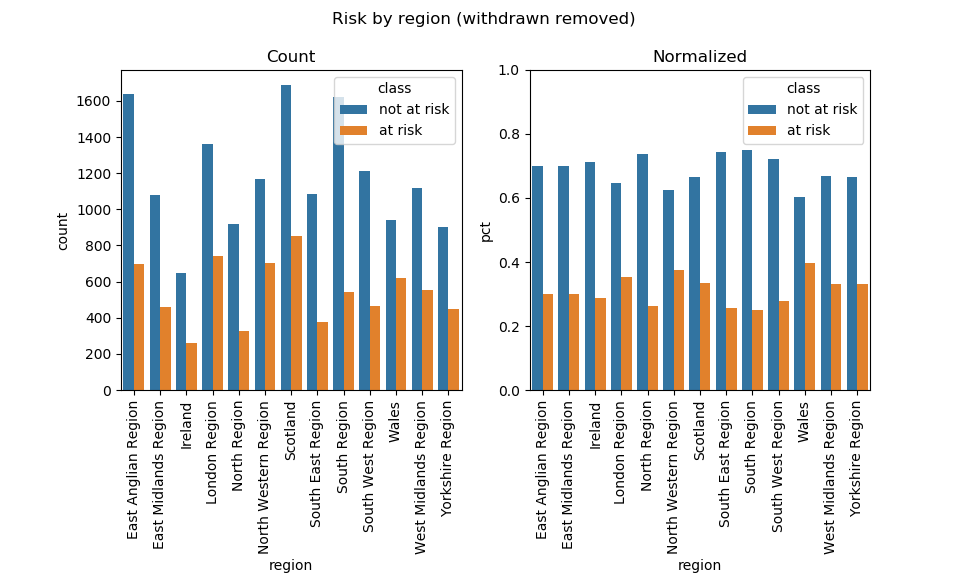
\includegraphics[width=0.8\textwidth]{EDA/withdrawn_not_at_risk/risk_by_region_combined.png}}
		\caption{Risk by region, count and normalized}
		\label{fig:risk_by_region_nowd}
	\end{subfigure}
	\caption{Risk by feature for failure only data}
	\label{fig:feature_risk_nowd}
\end{figure}
After removing students who had withdrawn the dataset become unbalanced with 32\% \texttt{at risk} and 68\% \texttt{not at risk}. Additionally, the apparent connection between features and risk changed. Age became a much stronger predictor, disability fell, region and highest education achieved remained strong indicators, however. This relationship is shown in Figure \ref{fig:feature_risk_nowd}

\begin{figure}[ht!]
	\centering
	\fbox{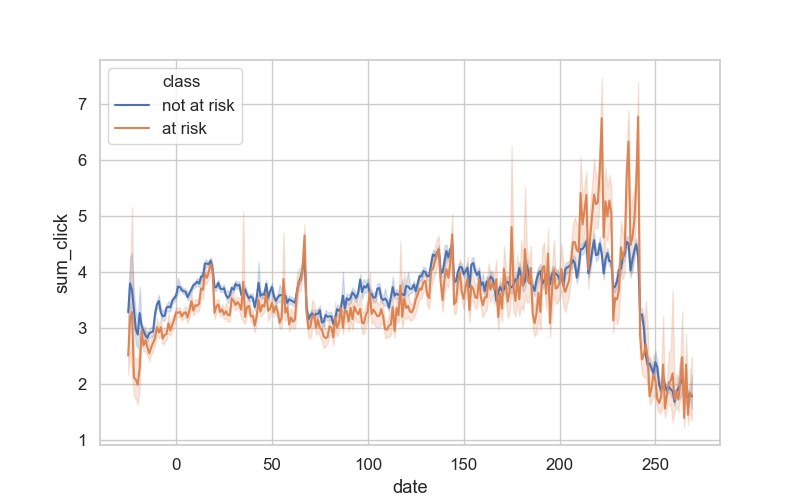
\includegraphics[width=0.8\textwidth]{EDA/withdrawn_not_at_risk/clicks_per_day.png}}
	\caption{Mean clicks per day (withdrawn removed)}
	\label{fig:clicks_per_day_nowd}
\end{figure}
Student activity exhibited an almost identical pattern with withdrawn students removed from the dataset (Figure \ref{fig:clicks_per_day_nowd}). This bore itself out during the experiments, and is discussed further in the conclusion.
\pagebreak[4]
\section{Experimental Setup and Data}
The data consists of 7 .csv files forming a database connecting student demographics, course data, assessment data, and VLE interaction click-stream data as shown in Figure \ref{fig:schema}. The problem will be modeled as a binary classification problem consisting of two classes: \texttt{at risk}, and \texttt{not at risk}. \texttt{studentinfo.csv} classifies students as \texttt{Distinction, Pass, Fail, Withdawn}. In all cases I have consolidated \texttt{pass}, and \texttt{distinction} into the single classification of \texttt{not at risk}. What consitutes risk however is not as straight forward. I have chosen to analyze the data in 2 ways:
\begin{figure}[ht!]
	\centering
	\fbox{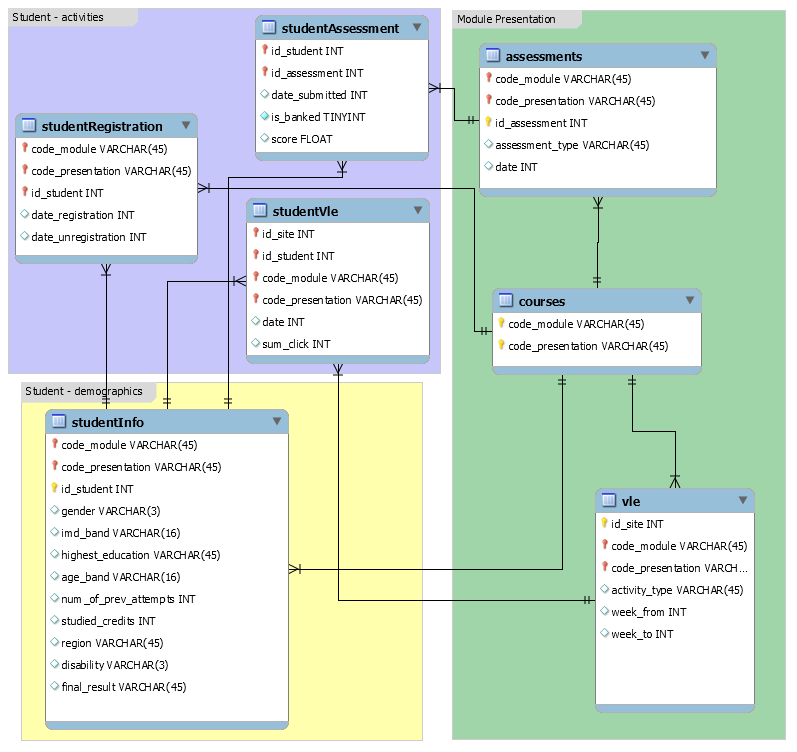
\includegraphics[width=0.45\textwidth]{images/database_model.png}}
	\caption{OULAD database schema}
	\label{fig:schema}
\end{figure}
\begin{itemize}
    	\item Withdrawn and failure $\rightarrow$ \texttt{at risk}
	\item Withdrawn removed; only failure $\rightarrow$ \texttt{at risk}
\end{itemize}

\subsection{Failure and Withdrawn \texttt{at risk}}
\texttt{studentinfo.csv} contains 32,593 instances with students who have withdrawn included. Of these 17,208 (53\%) are \texttt{at risk}, and 15,385 (47\%) are \texttt{not at risk}.
\subsubsection{Demographics}
A model was trained first with all features, and then recursive feature elimination was used.
\begin{center}
\begin{tabular}{|c|rr|}
\hline
\multirow{4}{10cm}{\textbf{Decision Tree}, all features, no pruning}
&F1:&  0.5300751596360103\\
&P:&   0.55853345228728\\
&R:&   0.5122745504163213\\
&ACC:& 0.5213455954803108\\
\hline
\multirow{4}{10cm}{\textbf{Decision Tree}, all features, pruned to depth = 3}
&F1:&   0.5960770313754884\\
&P:&   0.6084919709282606\\
&R:&   0.6010087413775903\\
&ACC:& 0.577632558938233\\
\hline
\multirow{4}{10cm}{\textbf{Logistic regression}, all features}
&F1:&  0.6033966349724211\\
&P:&   0.6002020723205602\\
&R:&   0.6521749970644297\\
&ACC:& 0.5698497943495411\\
\hline
\multirow{4}{10cm}{\textbf{Random Forest}, all features }
&F1:&  0.5885641454642756 \\
&P:&   0.5789355549279234 \\
&R:&   0.612470072634394 \\
&ACC:& 0.5513946255038854 \\
\hline
\multirow{4}{10cm}{\textbf{Random Forest}, all features, pruned to depth = 3}
&\textbf{F1}:&  \textbf{0.666812465970329} \\
&P:&   0.5723193485418702 \\
&R:&   0.8068065322396238 \\
&\textbf{ACC}:& \textbf{0.5721045993342264} \\
\hline
\hline
\hline
\multirow{4}{10cm}{\textbf{Decision Tree}, highest\_education, region, gender, disability, no pruning}
&F1:&  0.6194940570468739\\
&P:&   0.589318894225182\\
&R:&   0.6582959743400265\\
&ACC:& 0.5701985667526074\\
\hline
\multirow{4}{10cm}{\textbf{Decision Tree}, highest\_education, region, gender, disability, pruned to depth = 3. \textit{Illustrated in Figure \ref{fig:demographic_dtree_pruned}}}
&F1:&  0.5917318113490284\\
&P:&   0.5983365588565791\\
&R:&   0.594766915726622\\
&ACC:& 0.5652109402855962\\
\hline

\multirow{4}{10cm}{\textbf{Logistic regression}, highest\_education, region, gender, disability, no pruning }
&F1:&  0.5930103011463939 \\
&P:&   0.5806063792573536 \\
&R:&   0.6162824292218575 \\
&ACC:& 0.5549203559751633 \\
\hline
\multirow{4}{10cm}{\textbf{Random Forest}, highest\_education, region, gender, disability, no pruning }
&F1:&  0.6253177280985549 \\
&P:&   0.587579935347121 \\
&R:&   0.6793333033154727 \\
&ACC:& 0.5721054064792355 \\
\hline
\multirow{4}{10cm}{\textbf{Random Forest}, highest\_education, region, gender, disability, pruned to depth = 3}
&\textbf{F1}:&  \textbf{0.6579396580825498} \\
&P:&   0.5673330923414592 \\
&R:&   0.7921906240095209 \\
&\textbf{ACC}:& \textbf{0.5628288434883273} \\
\hline
\end{tabular}
\end{center}
\begin{figure}[ht!]
	\centering
	\fbox{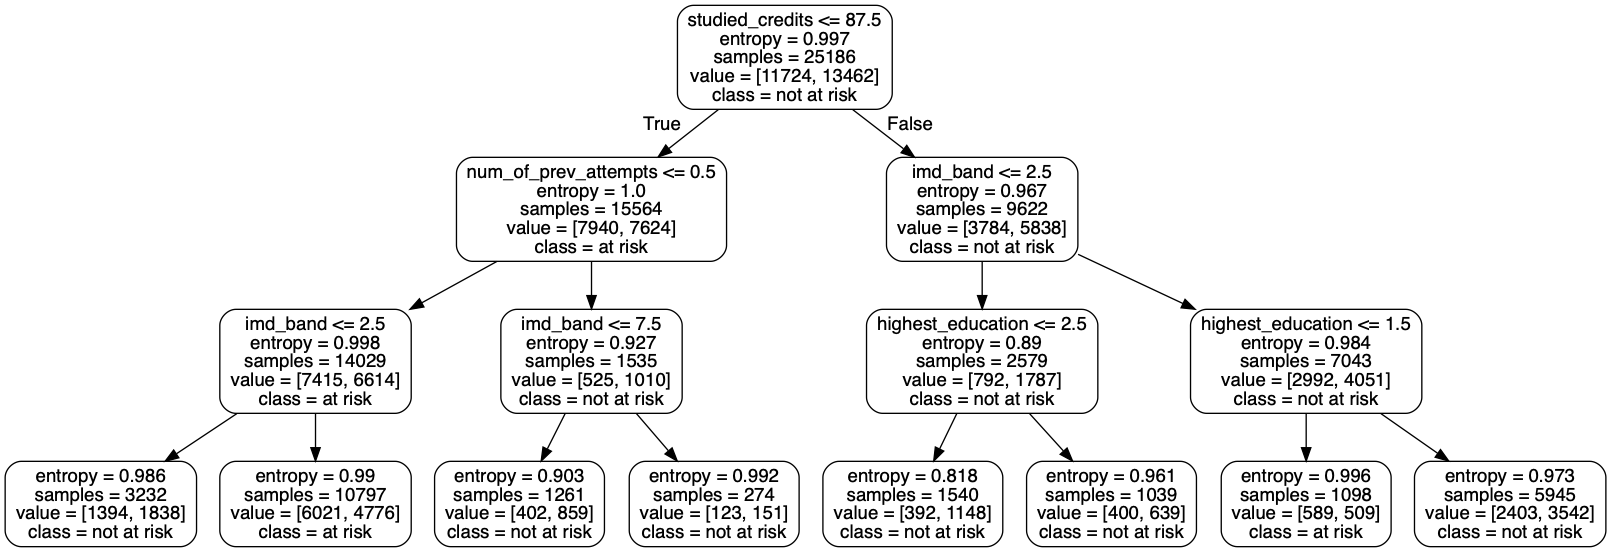
\includegraphics[width=1\textwidth]{images/dtree_pruned_all.png}}
	\caption{Demographic based decision tree classifier (withdrawn at risk)}
	\label{fig:demographic_dtree_pruned}
\end{figure}

\subsubsection{VLE Interaction}
\begin{center}
\begin{tabular}{|c|rr|}
\hline
\multirow{4}{10cm}{\textbf{Logistic Regression}, clicks per day}
&F1:&  0.7851064207596459\\
&P:&   0.7206436088430447\\
&R:&   0.862602495543672\\
&ACC:& 0.7690144139280324\\
\hline
\multirow{4}{10cm}{\textbf{SVM}, mean clicks per day}
&F1:&  0.8415578470397914 \\
&P:&   0.8992202025711 \\
&R:&   0.7911586452762924 \\
&ACC:& 0.8544488198550825 \\
\hline
\multirow{4}{10cm}{\textbf{Logistic Regression}, binary activity per day}
&F1&:  0.8302630656926905\\
&P:&   0.8076095227708657\\
&R:&   0.8546880570409983\\
&ACC:& 0.8291667001054233\\
\hline
\multirow{4}{10cm}{\textbf{SVM}, binary activity per day}
&\textbf{F1}:&  \textbf{0.8561210723707424} \\
&P:&   0.9334441815817172 \\
&R:&   0.7910873440285205 \\
&\textbf{ACC}:& \textbf{0.8701753893183237} \\
\hline
\end{tabular}
\end{center}
\subsection{Only failure \texttt{at risk}}
It is reasonable that students who withdraw and students who fail face different stressors, and their demographics and behaviors may not align. By removing students who withdraw and treating just those that fail separately I attempt to show that we can increase classification performance. \texttt{studentinfo.csv} contains 21,562 instances with students who have withdrawn included. Of these 6907 (32\%) are \texttt{at risk}, and 14,655 (68\%) are \texttt{not at risk}.
\subsubsection{Demographics}
\begin{center}
\begin{tabular}{|c|rr|}
    \hline
    \multirow{4}{10cm}{\textbf{Decision Tree}, all features, no pruning}
&F1:&  0.3551014504455618\\
&P:&   0.34250211116095125\\
&R:&   0.4012139109330578\\
&ACC:& 0.5507328880585811\\
\hline
\multirow{4}{10cm}{\textbf{Decision Tree}, all features, pruned to depth = 3}
&F1:&  0.1942524477422683 \\
&P:&   0.39739679699001756 \\
&R:&   0.1708584877880602 \\
&ACC:& 0.6369959633622646 \\
\hline
\multirow{4}{10cm}{\textbf{Logistic regression, all features}}
&F1:&  0.22522736170125715\\
&P:&  0.47607224321518354\\
&R:&   0.19867322804528276\\
&ACC:& 0.6362534826969592\\
\hline
\multirow{4}{10cm}{\textbf{Random Forest}, all features }
&\textbf{F1}:&  \textbf{0.32633444850345555} \\
&P:&   0.3931869763753829  \\
&R:&   0.32897793184535634 \\
&\textbf{ACC}:& \textbf{0.6011449077238551} \\
\hline
\multirow{4}{10cm}{\textbf{Random Forest}, all features, pruned to depth = 3}
&F1:&  0.0906114249018504 \\
&P:&   0.6657277830429393 \\
&R:&   0.10079453320911984 \\
&ACC:& 0.637645593616744 \\
\hline
\hline
\hline
\multirow{4}{10cm}{\textbf{Decision Tree}, highest\_education, region, gender, disability, no pruning}
&F1:&  0.11241468166145423\\
&P:&   0.5135856539476726\\
&R:&   0.06559562220794721\\
&ACC:& 0.6790648886074675\\
\hline
\multirow{4}{10cm}{\textbf{Decision Tree}, highest\_education, region, gender, disability, pruned to depth = 3. \textit{Illustrated in Figure \ref{fig:demographic_dtree_pruned_nowd}}.}
&F1:&  0.09857606225251082\\
&P:&   0.5280882756223184\\
&R:&   0.05486889992465453\\
&ACC:& 0.6808275408470831\\
\hline
\multirow{4}{10cm}{\textbf{Logistic regression}, RFE}
&F1:&  0.22326091573672335\\
&P:&   0.44777700838143647\\
&R:&   0.19403827633869203\\
&ACC:& 0.6307807930203678\\
\hline
\multirow{4}{10cm}{\textbf{Random Forest}, RFE, no pruning }
&F1:&  0.30227509353062393 \\
&P:&   0.33621906995183387 \\
&R:&   0.32723513551182004 \\
&ACC:& 0.566594144982572 \\
\hline
\multirow{4}{10cm}{\textbf{Random Forest}, RFE, pruned to depth = 3}
&\textbf{F1}:&  \textbf{0.14339788733546183} \\
&P:&   0.5248863556150724 \\
&R:& 0.13742217881503263 \\
&\textbf{ACC}:& \textbf{0.640427955006803} \\
\hline
\end{tabular}
\end{center}
\begin{figure}[ht!]
	\centering
	\fbox{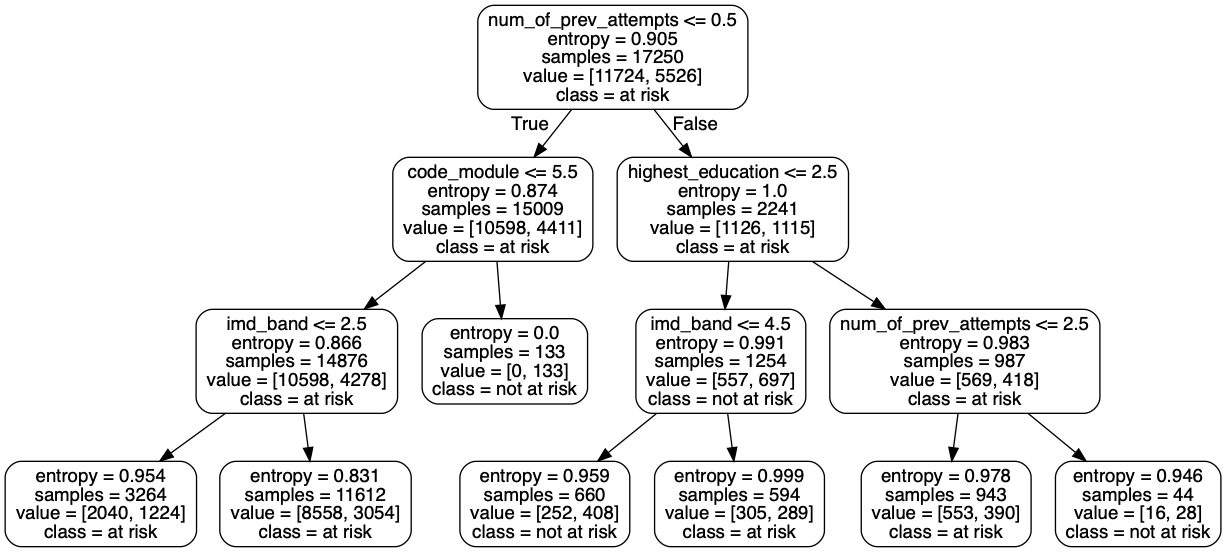
\includegraphics[width=1\textwidth]{images/dtree_pruned_nowd.png}}
	\caption{Demographic based decision tree classifier (withdrawn not at risk)}
	\label{fig:demographic_dtree_pruned_nowd}
\end{figure}

\subsubsection{VLE Interaction}
\begin{center}
\begin{tabular}{|c|rr|}
\hline
\multirow{4}{10cm}{\textbf{Logistic Regression}, mean clicks per day}
&F1:&  0.715838193171871\\
&P:&   0.7212950509072961\\
&R:&   0.7114608832840876\\
&ACC:& 0.7980088914969958\\
\hline
\multirow{4}{10cm}{\textbf{SVM}, mean clicks per day}
&F1:&  0.7220974641305407 \\
&P:&   0.8226623239904555 \\
&R:&   0.6439019883771265 \\
&ACC:& 0.8228411121874819 \\
\hline
\multirow{4}{10cm}{\textbf{Logistic Regression}, binary activity per day}
&F1:&  0.7316291147828424\\
&P:&   0.7492935584330797\\
&R:&   0.7152688600202411\\
&ACC:& 0.8124427477588576\\
\hline
\multirow{4}{10cm}{\textbf{SVM}, binary activity per day}
&\textbf{F1}:&  \textbf{0.7413424042386404} \\
&P:&   0.8826494386069681 \\
&R:&   0.6393569109038723 \\
&\textbf{ACC}:& \textbf{0.840609158133932} \\
\hline
\end{tabular}
\end{center}

\pagebreak[4]
\section{Results}
\begin{figure}[ht!]
	\centering
	\fbox{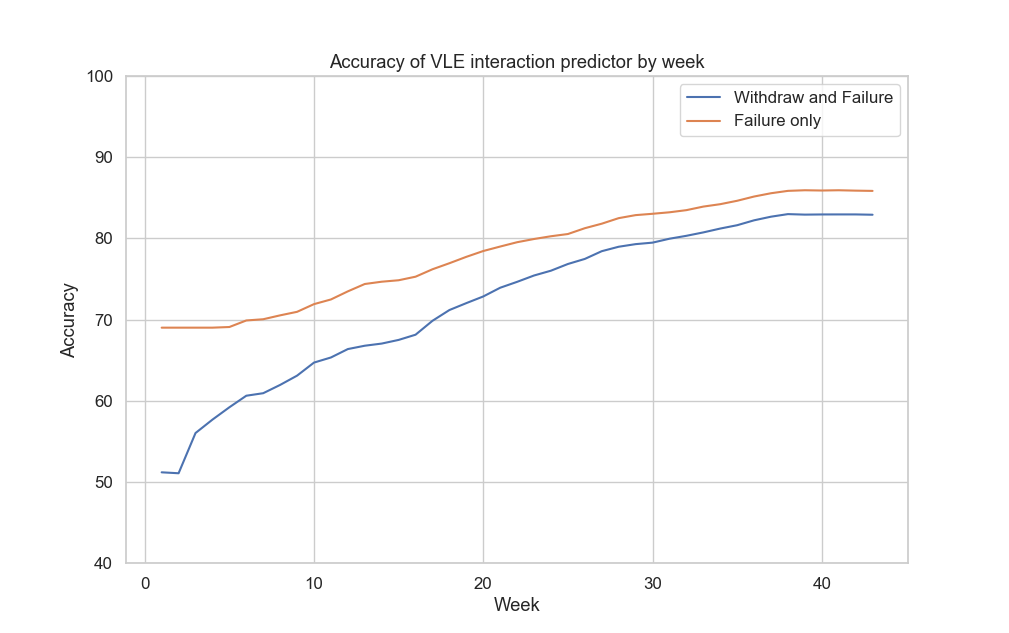
\includegraphics[width=1\textwidth]{images/accuracy_per_week.png}}
	\caption{Change in accuracy of classifier over length of course}
	\label{fig:accuracy_per_week}
\end{figure}
The goal of this study was to find a means for learning administrators to identify students at risk of failing prior to the end of the course. \ref{fig:accuracy_per_week} shows the increase in accuracy of the binary linear regression models as time increases. By week 20 the system is able to identify at risk students with over 70\% accuracy whether at risk is defined as withdraw and failure, or solely at risk of failure. The model which only predicts failure performs with a higher accuracy, but both can aide schools at assisting students, and can be used in concert.

\section{Conclusion}
At the beginning of this experiment I thought that demographics would be a much stronger predictor of success than they turned out to be. The analysis concluded that simply tracking whether a user is frequently active, or not, is the strongest predictor of student success. This is good news for administrators, and developers developing software to identify at risk students. A simply binary log of daily activity is:
\begin{enumerate}
	\item Easy to develop
	\item Inexpensive to store
	\item Free of personal data
\end{enumerate}
Discriminating withdraws from failures also did not seem to be necessary for the binary activity classifier. Performance was comparable in both cases. This is good news for administrators interested in maximum retention. Although the causes of each case of non-completion may be different, the symptom of not being active can be identified either way. This allows for first level intervention, triage of sort, to identify what exactly is causing the student's lack of activity and help can be administered whether it be academic, social, or health related. Although SVM had the best performance, it was significantly slower to train than the other models, and its performance gains were modest compared to logistic regression.


\section{Future work}
Although in this paper I showed that it is a possible, and practical task for learning environment administrators to use data mining techniques to identify at risk students, the work is by no means conclusive or complete. A notable absence is investigation of applying unsupervised learning techniques to this problem. A potential system could use clustering to the activity data in an attempt to identify types of users. It is conceivable that users fall into discrete activity levels, each exhibiting a similar level of risk. This is not explored in this paper, but is a potential area of future work.\\

Finally, the work has shown that separating withdraw risk from failure risk yields dividends. It would be a worthy use of time to perform this analysis and identify withdraw risk separate from failure risk and develop an independent classifier to help students at risk of withdrawing.

\end{document}
